%!TEX root = ../thesis.tex
%*******************************************************************************
%*********************************** First Chapter *****************************
%*******************************************************************************

\chapter{Correlations of the impedance plethysmography device}  %Title of the First Chapter
\label{chapter correlations}
\ifpdf
    \graphicspath{{Chapter6/Figs/Raster/}{Chapter6/Figs/PDF/}{Chapter6/Figs/}}
\else
    \graphicspath{{Chapter6/Figs/Vector/}{Chapter6/Figs/}}
\fi

The previous chapter \ref{chapter results} showed the performance of the designed impedance plethysmography device and the data collected in resistivity value and its equivalent in blood flow. It was shown the capability of the instrument on detecting changes during three different kinds of occlusion. Furthermore, it was presented the data collected from the other devices such as ultrasound Doppler, LDF, PPG and ECG. 

In this chapter, the correlation between the different measurements gathered will be analysed. The aim of this correlational investigation is understanding what the contributing factors towards the impedance plethysmography signal are. As it has been explained in previous chapters, the change of the volume in the forearm section let to estimate the blood flow from the segment. However, both arterial and venous blood contributes to the information of blood flow calculated by the iPG device. It is not clear, how much of the blood flow belongs to any of the types of blood. Besides, it was shown that main blood vessels contribute to the measurement of blood flow but microcirculation might also provide additional information under the iPG waveform. 

\mynote{This paragraph is quite an statement. I have to verify if I can really calculate how much is the contribution of the micro circulation and the other types of blood flow.}

%********************************** %First Section  **************************************
\section{Analysis of the the heart beat detection in the frequency domain} %Section - 6.1
\label{section correlation 1} 
The signals obtained from all the devices during the experiment are synchronous to the heart beat. This synchronisation reflects that in their dynamic component the systolic peak is also present in the waveform of these instruments.

Nonetheless, some noises impact negatively to the proper detection of the systolic peaks during the study. The algorithm designed can detect the shape of the waveform by finding the foot of the signal and its peaks. Nevertheless, some of the peaks might be missing because of the noise levels.

A Fast Fourier Transform was used to detect the main harmonic of the waveforms in a random window data set. The data selected was between \SIrange{580}{780}{\second} for the AC components only. The algorithm was programmed to detect the frequency peak ($f_p$) from \SIrange{0.85}{1.75}{\hertz}. The FFT was limited to detected frequencies between \SIrange{0}{5}{\hertz} due to the filters applied to the waveforms as explained in section \ref{section procedure 3}.

From Figure \ref{fig:fft signals} can be seen the frequency components from all participants measurements. The ECG plots show the frequency response typical of this kind of signal. Some signals presented a high level of high-frequency components such as the ones seen in participants 1 and 8. The Participant 3 showed a high \SI{2}{\hertz} harmonic peak which power was greater than the first harmonic. This response seems odd but by examining the waveform in detail showed a lower Q wave which might influence the abnormal frequency component presented in the graph.

The iPG device had a mixed frequency response to detecting the cardiac heartbeat. As it can be seen from the shown plots, some signals show a low-frequency noise which in some cases it is larger than the expected first harmonic. For instance, participants 1, 3 4 and 6 was hard to detect the frequency peak related to the cardiac cycle for this particular data set. However, the rest of the partakers registered a frequency peak at similar heart beat as the ECG. 

PPG frequency components were quite clear in all the participants. Some of them showed high-frequency noise as participant 8. However, in general, this signal shows low signal to noise ration compared to iPG which is understandable as the PPG-AC is significantly larger than the iPG-AC amplitude

Lastly, UD exhibited a clear FFT components in most of the participants. Only Participant 1 demonstrated a high noise component in his measurements but the rest showed a response similar to the ECG. 

Table \ref{tbl:fft} demonstrates how close the cardiac frequency is to each instrument. However, the iPG mean harmonic and frequency distribution from participant 8 illustrates that his data was not clean.


\begin{figure}[!htpb]
	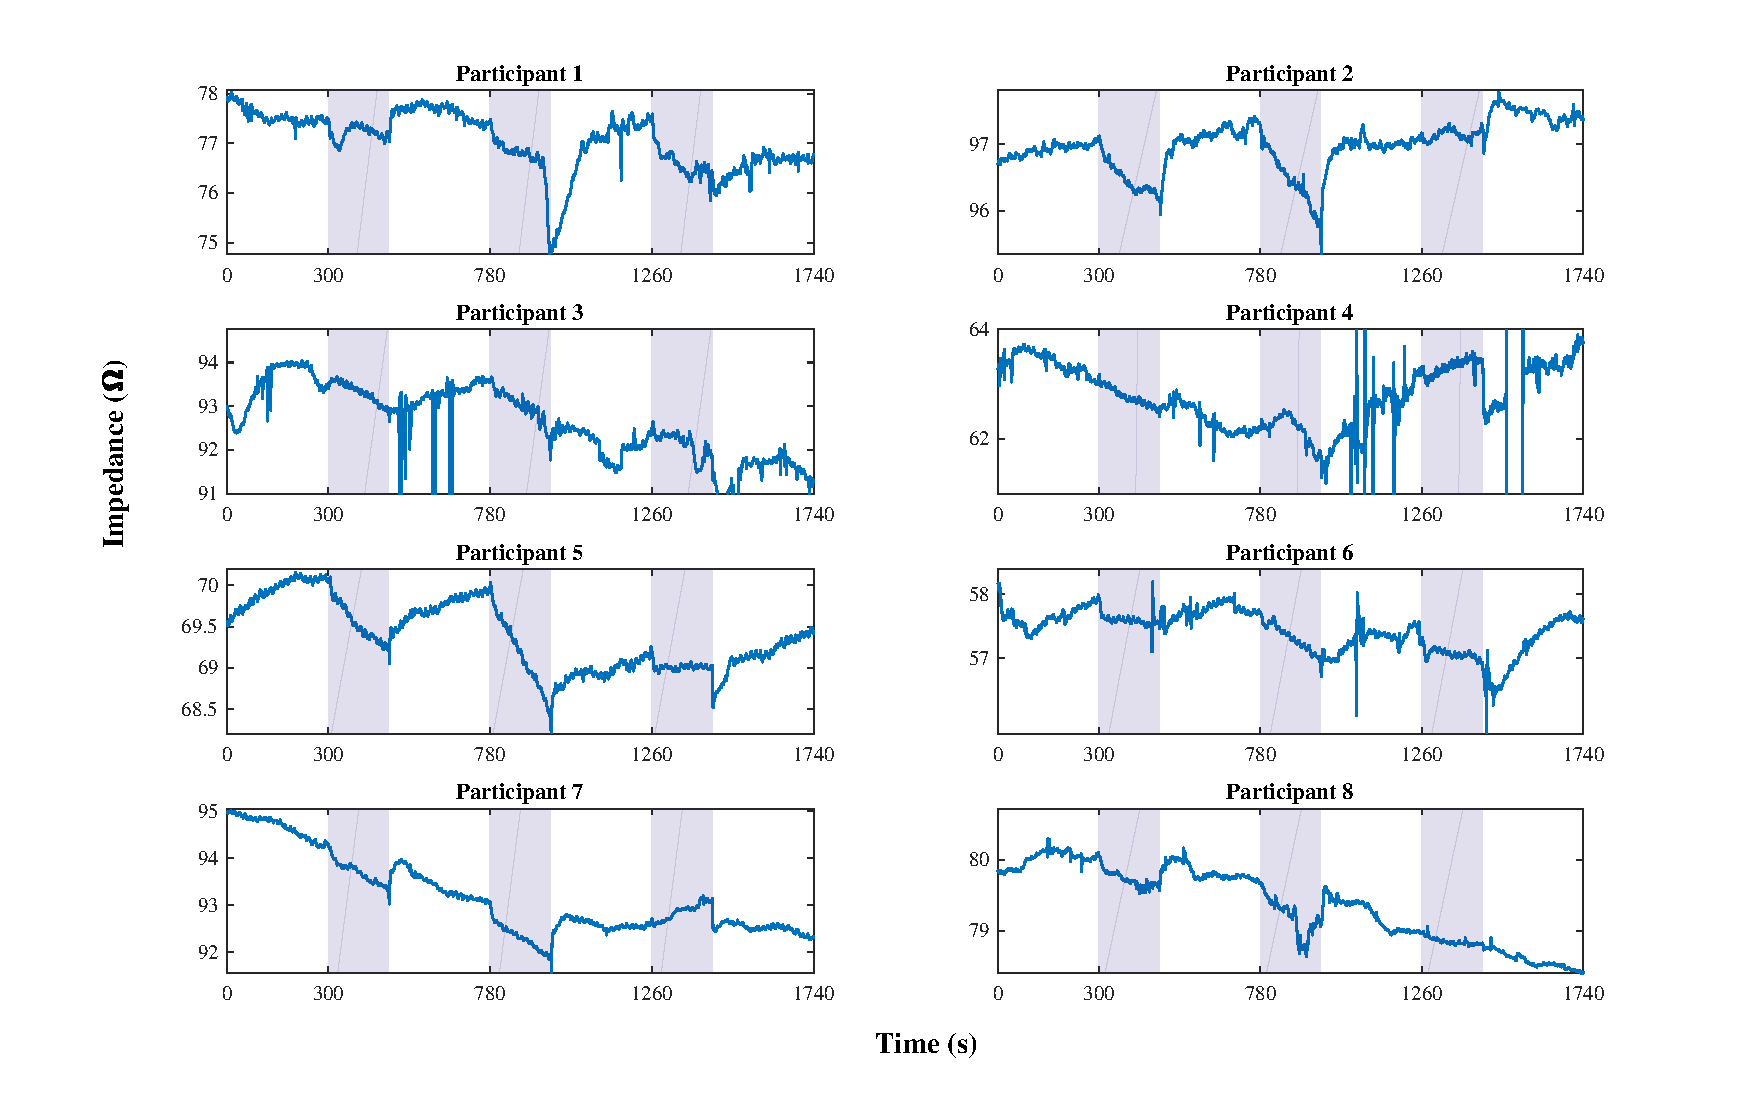
\includegraphics[width=1\textwidth,keepaspectratio,trim={0.75cm 0cm 2cm 2cm},clip]{figure1}    
	\caption[Fequency components of the signals acquired]{Blood flow calculated from venous occlusion plethysmography}
	\label{fig:fft signals}
\end{figure}

\begin{table}[!htbp]
	\caption[Peak frequency calculated obtained form Fast Fourier Transform]{Cardiac frequency obtained from the Fast Fourier Transform for each of the instruments used during the experiment. This peak corresponds to the one with in the hearth cycle in the study (\SI{0.5}{\hertz} < $f_p$ > \SI{1.5}{\hertz})}
	\label{tbl:fft}
	\centering 
	\begin{tabular}{lccccc}
		\toprule
		& \textbf{ECG}
		& \textbf{iPG}
		& \textbf{PPG}
		& \textbf{LDF}
		& \textbf{UD} \\
		& \textbf{$f_p$ [\si{\hertz}]}		
		& \textbf{$f_p$ [\si{\hertz}]}		
		& \textbf{$f_p$ [\si{\hertz}]}
		& \textbf{$f_p$ [\si{\hertz}]}
		& \textbf{$f_p$ [\si{\hertz}]}\\\midrule
	    Participant 1    &     0.967    &     0.952    &     0.949    &     0.897    &     0.949    \\  
		Participant 2    &     0.964    &     0.964    &     0.989    &     0.964    &     0.964    \\  
		Participant 3    &     1.041    &     0.916    &     1.041    &     1.038    &     1.019    \\  
		Participant 4    &     1.425    &     1.437    &     1.422    &     1.321    &     1.425    \\  
		Participant 5    &     0.940    &     0.940    &     0.937    &     0.940    &     0.940    \\  
		Participant 6    &     1.239    &     1.242    &     1.242    &     1.233    &     1.239    \\  
		Participant 7    &     1.163    &     1.163    &     1.163    &     1.163    &     1.163    \\  
		Participant 8    &     1.346    &     1.401    &     1.337    &     1.367    &     N/A    \\  
 
	\bottomrule
	\end{tabular}
\end{table}


%********************************** %Second Section  *************************************
\section{Why do we use loren ipsum?} %Section - 6.2
\label{section correlation 2} 

%********************************** % Third Section  *************************************
\section{Where does it come from?}  %Section - 6.3 
\label{section correlation 3}

